\documentclass[10pt]{beamer}
\usepackage{appendixnumberbeamer}
\usepackage{booktabs}
\usepackage[scale=2]{ccicons}
\usepackage{amsmath}
\usepackage{pgfplots}
\usepackage[backend=biber]{biblatex}
\usepackage{xspace}
\usepackage{caption}
\usepackage{subcaption}

\usetheme[progressbar=frametitle]{metropolis}
\setbeamercolor{background canvas}{bg=white}
\usepgfplotslibrary{dateplot}
\addbibresource{demo.bib}

\newcommand{\themename}{\textbf{\textsc{metropolis}}\xspace}
\newcommand\Wider[2][3em]{%
\makebox[\linewidth][c]{%
  \begin{minipage}{\dimexpr\textwidth+#1\relax}
  \raggedright#2
  \end{minipage}%
  }%
}

\title{Final Project - Epidemic spreads over the flight network}
\date{\today}
\author{Marlene Funke (15-738-719), Aleksandar Novković (16-733-032),\\Sandra Trachsel (15-718-190), Miguel Vázquez (16-712-598)}
\institute{Network Science, Faculty of Business, Economics and Informatics\\Prof. Dr. Claudio Tessone}
\titlegraphic{\hfill
\includegraphics[height=1.5cm]{Template_resources/uzh_logo_d_pos.pdf}}

\begin{document}
\maketitle

\section{Introduction}
\begin{frame}{Context}
    \begin{figure}
        \begin{center} 
        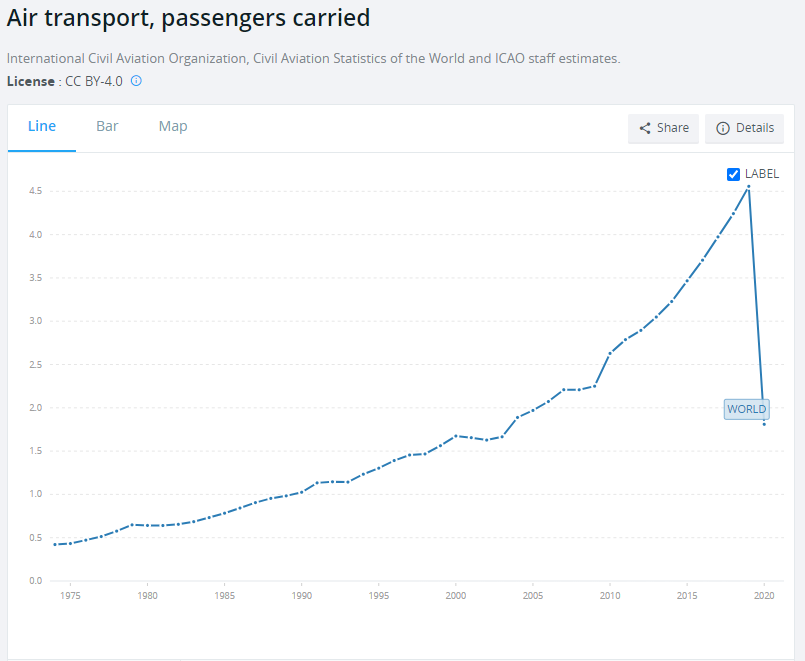
\includegraphics[width=0.8\textwidth]{Figures/Air_transport.png}
        \end{center}
    \end{figure}
\end{frame}
\begin{frame}{Goals}
    \begin{itemize}\itemsep2em
        \item Rank different centrality measures, based on different outcomes of interest, by their ability to properly identify and shut down spreader nodes as to avoid a new pandemic taking over through the world airline network
        \item Understand how much the different centrality measures correlate with each other
    \end{itemize}
\end{frame}
\begin{frame}{Questions}
    \begin{itemize}\itemsep2em
        \item Is there a definite best centrality measure to achieve our goal?
        \item If yes, which one (of the ones we selected) is it?
        \item If no, does it depend on the outcome or on the governmental allowance? Or both?
    \end{itemize}
\end{frame}



\section{Model}
\begin{frame}{5 Centrality Measures}
    \begin{itemize}
        \item Betweenness centrality
        \begin{itemize}
            \item Shortest paths between all pairs of nodes in a graph
        \end{itemize}
            \item Eigenvector centrality
        \begin{itemize}
            \item Assigns a relative value to a node with respect to the nodes it is connected to
        \end{itemize}
        \item Closeness centrality
        \begin{itemize}
            \item Shortest distance of a node to all other nodes
        \end{itemize}
        \item In-degree centrality
        \begin{itemize}
            \item Number of arrival flights
        \end{itemize}
        \item Out-degree centrality
        \begin{itemize}
            \item Number of departure flights
        \end{itemize}
    \end{itemize}
\end{frame}
\begin{frame}{4 Outcomes of Interest}
    \begin{itemize}\itemsep2em
        \item Height of infection peak \\
        \item Total number of infections \\
        \item Time until peak reached \\
        \item Total epidemic length \\
    \end{itemize}
\end{frame}
\begin{frame}{Model Assumptions}
    \begin{itemize}
        \item Nodes $\rightarrow$ Airports  \\
        \item Edges $\rightarrow$ Routes (weighted by \# of airlines on that route $\times$ \# of seats on plane type used by that airline on that route).\\
        \item Same aircraft models have same \# of seats (no cargo shipping airplanes)\\
        \item One flight per route and period\\
        \item SIR model
        \item Infection rate = 0.005\\
        \item Recovery rate = 0.5 \\
        \item Airports are shut down after 0.5\% of nodes have been infected
        \item Selected airports will shut down completely and at the same time
    \end{itemize}
\end{frame}



\section{Data}
\begin{frame}{Raw Data}
OpenFlights.org GitHub repository:
    \begin{itemize}
        \item airports.dat
        \begin{itemize}
            \item 7,697 hubs, uniquely identified by ICAO code
        \end{itemize}
        \item routes.dat
        \begin{itemize}
            \item 67,663 connections, are uniquely identified by airline code - departure airport IATA code - arrival airport IATA code
        \end{itemize}
        \item planes.dat
        \begin{itemize}
            \item 246 aircrafts, uniquely identified by the airplane name
        \end{itemize}
    \end{itemize}
\end{frame}
\begin{frame}{Data Preparation}
    \begin{itemize}
        \item Matching routes and airports: adding coordinates
        \begin{itemize}
            \item 3,260 out of 3,422 (95\%) airports instantly matched
            \item 29 out of remaining 162 manually matched (IATA imputation)
            \item 133 remaining airports are discarded (=497 edges, $\sim$0.75\%)
            \item Further dropping 5 isolated airports
        \end{itemize}
        \item Adding weights
        \begin{itemize}
            \item WorldTrading.net to get most flight capacity estimates
            \item SeatLink.com to unify seats for same-model aircrafts
            \item Wikipedia.org for the remaining missing seats
        \end{itemize}
        \item Network simplification
        \begin{itemize}
            \item From multi-directed graph to simple directed graph
            \item 45\% edge compression
        \end{itemize}
    \end{itemize}
\end{frame}
\begin{frame}{Final Network}
\Wider[4em]{
    \begin{figure}
        \begin{center} 
        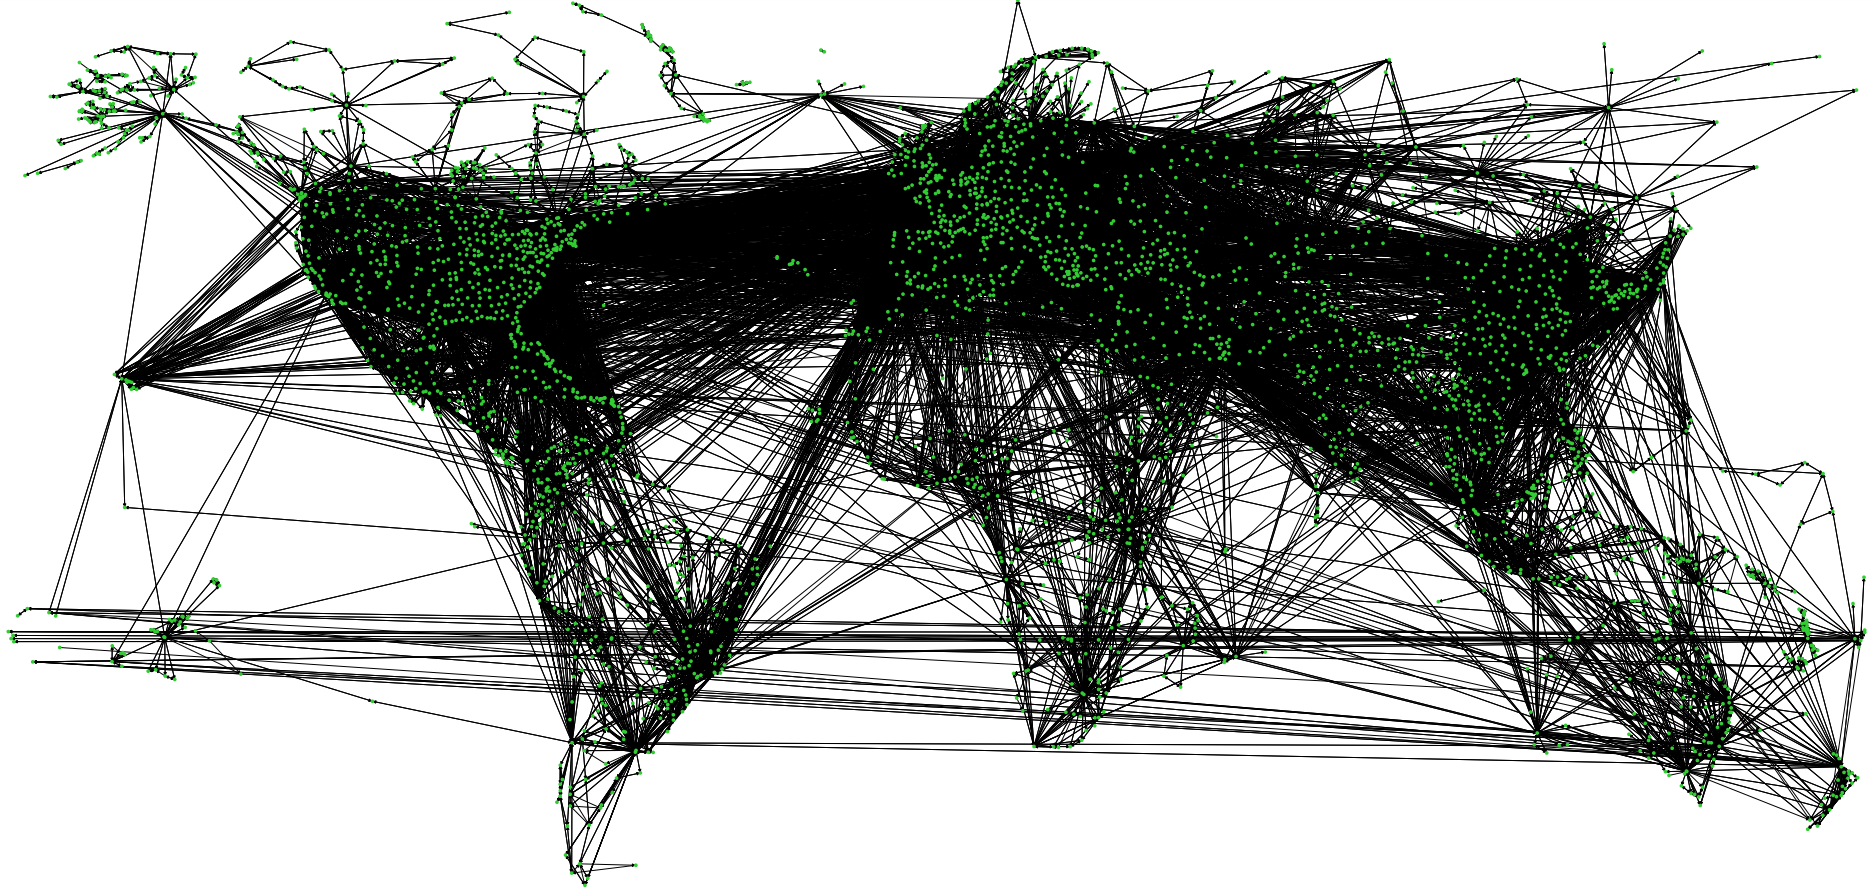
\includegraphics[width=\textwidth]{Figures/net_png.png}
        \newline3,284 nodes and 37,189 edges
        \end{center}
    \end{figure}
    }

\end{frame}




\section{Methods}

\begin{frame}{Analysis}
We simulated the pandemics in our network using the EoN package for Python
\begin{itemize}    
\item Epidemics of Networks
\item Using the SIR-Model for simulations
\item Many possible modules within the package to simulate pandemics apart from SIR
\item Since our computational power, our time and the scope of this project are limited, we decided to use the simple fast-SIR module

 \end{itemize}
\end{frame}

\begin{frame}{Fast-SIR}
\begin{itemize}    
\item This module implements the basic SIR-model
\item Uses, as seen in lecture, an ODE-model to obtain the simulation for each component (S, I and R) with respect to time-points
\item Parameters of the simulation are defined by the user 
\item Constant and exponentially distributed transmission and recovery rates (continous-time Markov chain)
\item Rather fast computation per simulation
 \end{itemize}
\end{frame}

\begin{frame}{Issues with Fast-SIR}
\begin{itemize}    
\item Fast-SIR returned very inconsistent arrays of time steps and thus outcomes of interest
\begin{itemize}
     \item Function solves equations continuously
     \end{itemize}
\item Need to align obtained simulations in order to construct averages and standard errors
\item t-steps need to be uniform and consistent
\item Linear interpolation used, which reconstructs the simulated pandemic

 \end{itemize}
\end{frame}

\begin{frame}{Interpolation of the Simulations Using Scipy}
\begin{figure}
\begin{center}
    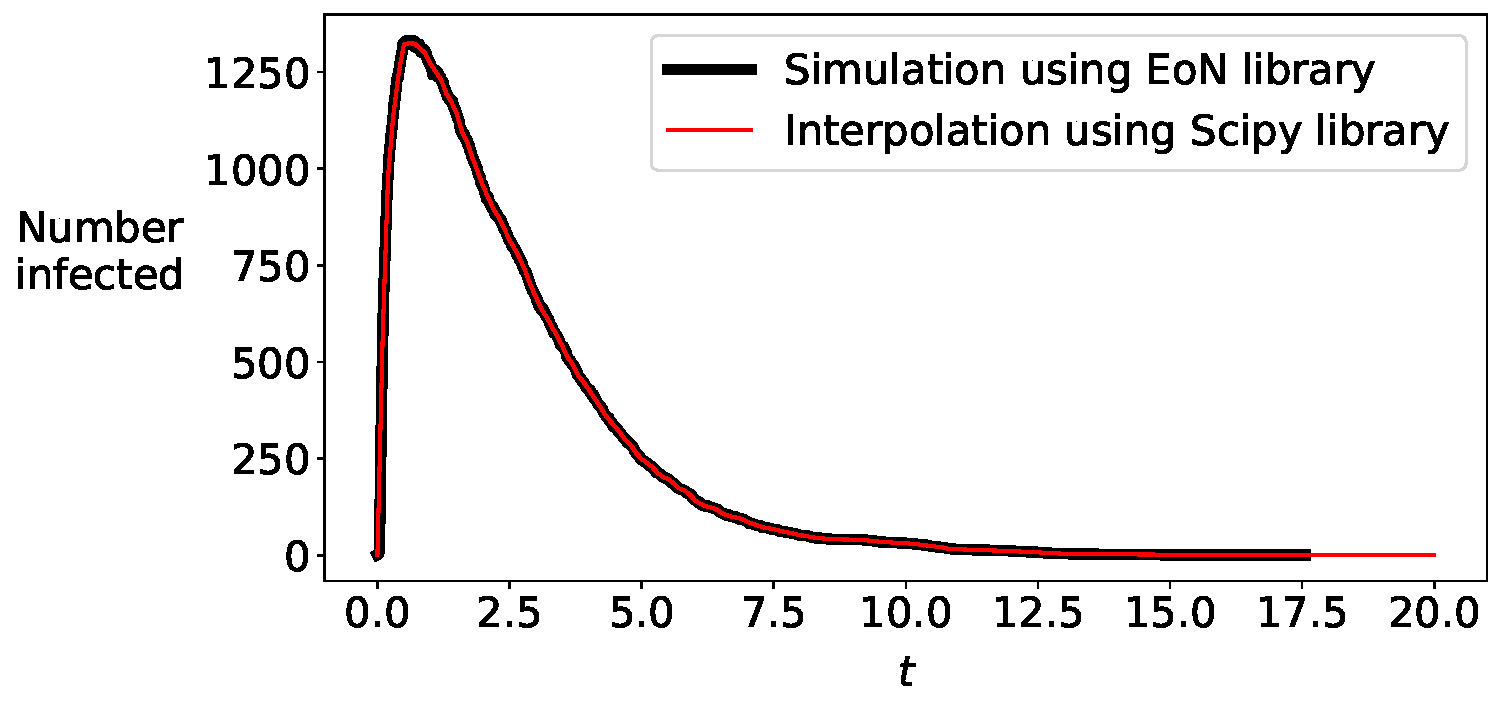
\includegraphics[width=0.8\textwidth]{Figures/interpolation_test.pdf}
\end{center}
\end{figure}
\end{frame}

\begin{frame}{Constructed counterfactual networks}
\begin{itemize}
\item Want to analyse the spread of a disease in the network when 'important' nodes are removed
\item Five different centrality measures to detect 'important' nodes
\item We constructed different scenarios which are equivalent to different degrees of node-removals
\begin{itemize}
     \item Removing individual sets of airports according to topX\% obtained from centrality measures (models governmental allowance)
     \item 12 different topX\% airports sets, ranging from top 1\% to top 12\%
     \item top 1\%: 33 nodes removed, top 12\%: 394 nodes removed
     \end{itemize}
\item In total we constructed 60 different scenarios of protective measures (5 measures $\times$ 12 sets of airports removed)
 \end{itemize}
\end{frame}

\begin{frame}{Simulations}
\begin{itemize}
\item We ran 100 simulations for each centrality measure with their topX\% remove plus the baseline network
\item Total of 7200 simulations (100 $\times$ 6 $\times$ 12)
\item Computed averages and standard errors across each cluster for four different outcomes of interest:
\begin{itemize}
     \item Height of peak
     \item Total number of infected people
     \item Time until peak
     \item Total length of pandemic
     \end{itemize}
 \end{itemize}
\end{frame}

\begin{frame}{Robustness of Simulations witch Concern to Parameters}
\begin{itemize}
\item We checked the robustness of our findings for different values of the recovery and transmission rate 
\item All tuples combining each of 3 recovery rates (0.1, 0.2, 0.3) with 3 transmission rates (0.1, 0.2, 0.4) were fed to the simulation
\item Findings: parameters do not change the relative ranking of the different measures
\begin{itemize}
     \item Only the absolute numbers of the pandemics change (total number infected, length of pandemic, etc.)
     \end{itemize}

\item Since we mostly focus on the relative difference between the measures and not the simulation itself (in terms of absolute numbers), the parameters remained the same throughout this analysis, as mentioned in the model assumptions

 \end{itemize}
\end{frame}



\section{Results and Discussion}

\begin{frame}{Comparing Centrality Measures}
\begin{figure}[!h]
    \begin{subfigure}[t]{0.45\textwidth}
        \centering
        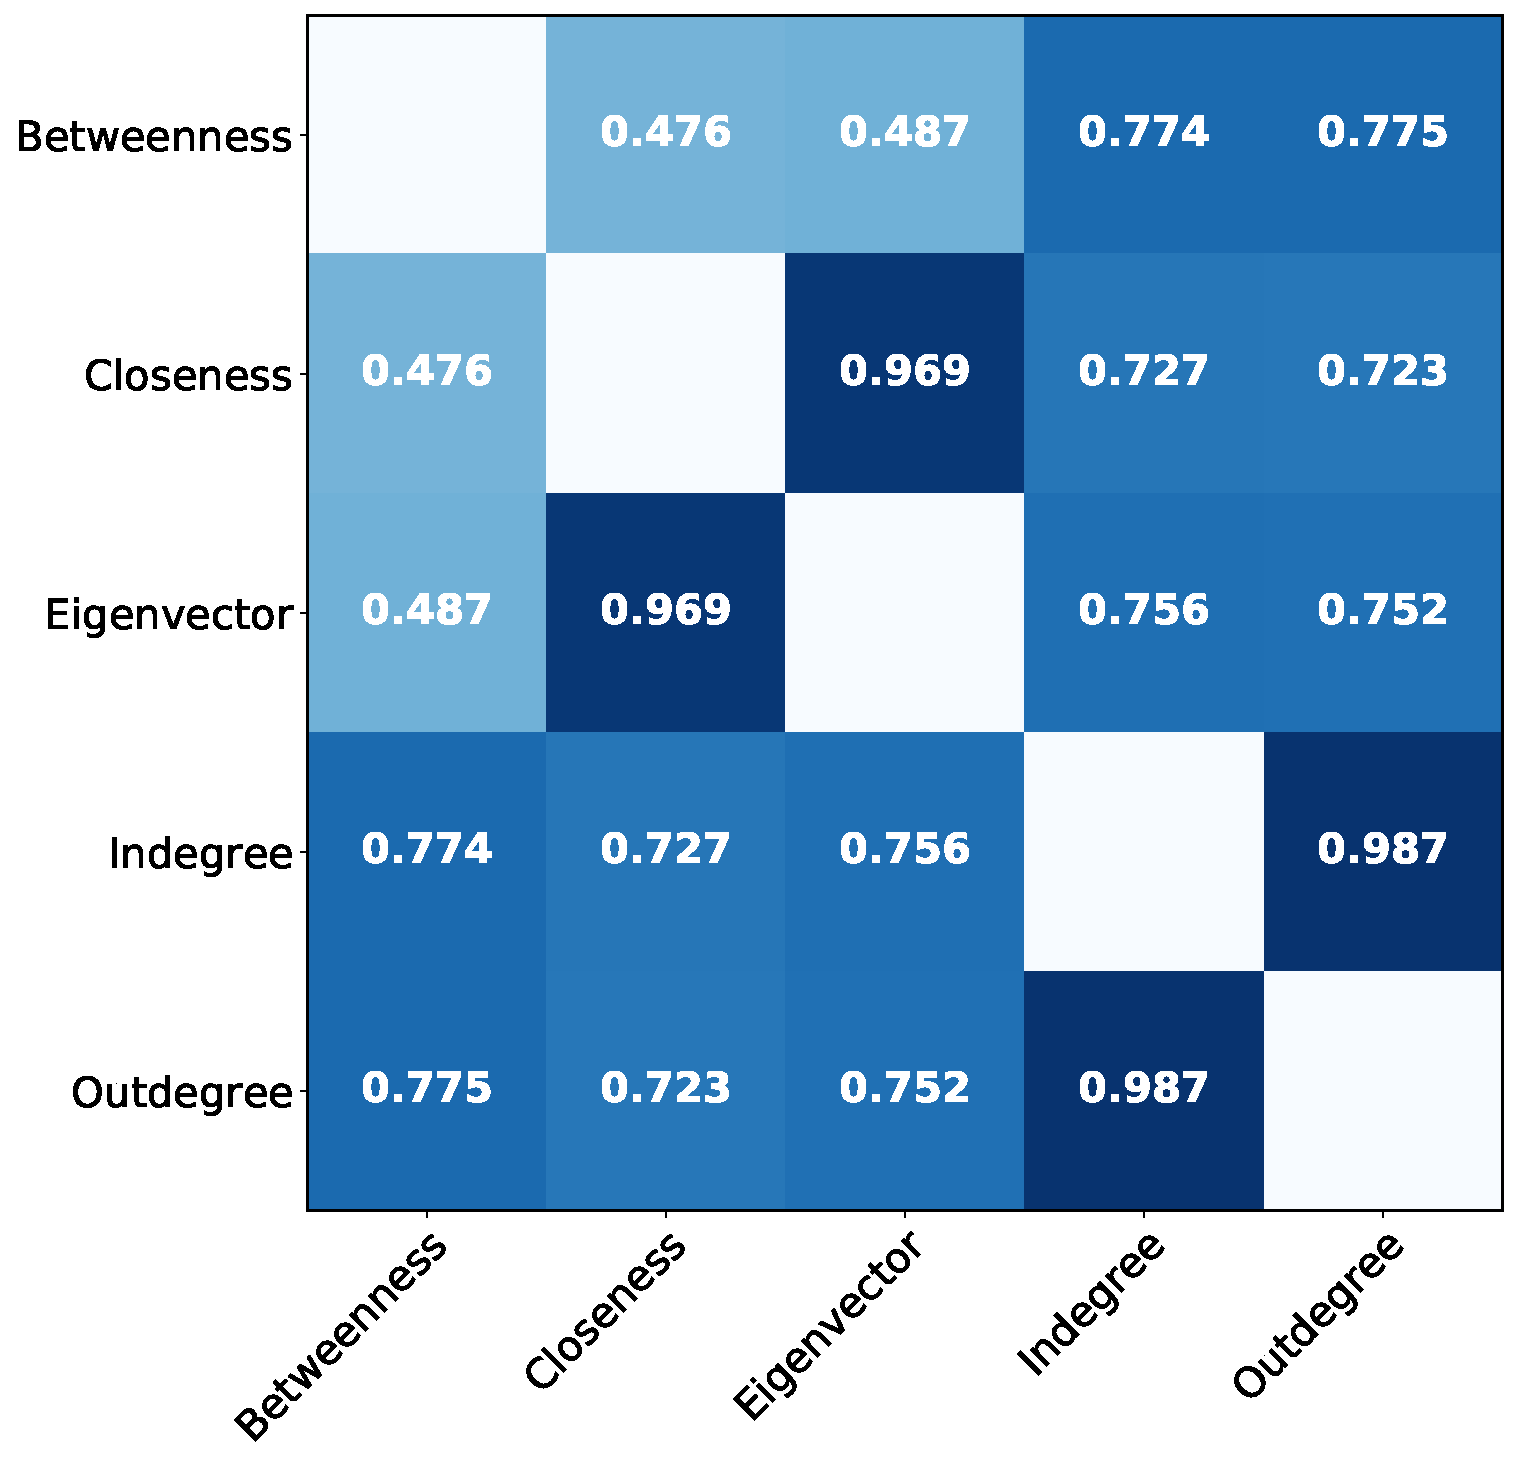
\includegraphics[width=1\textwidth]{Figures/spearman_matrix.pdf}
        \caption{Spearman}
        \label{fig:spearman_matrix}
    \end{subfigure}
    %\hfill
    \begin{subfigure}[t]{0.45\textwidth}
        \centering
        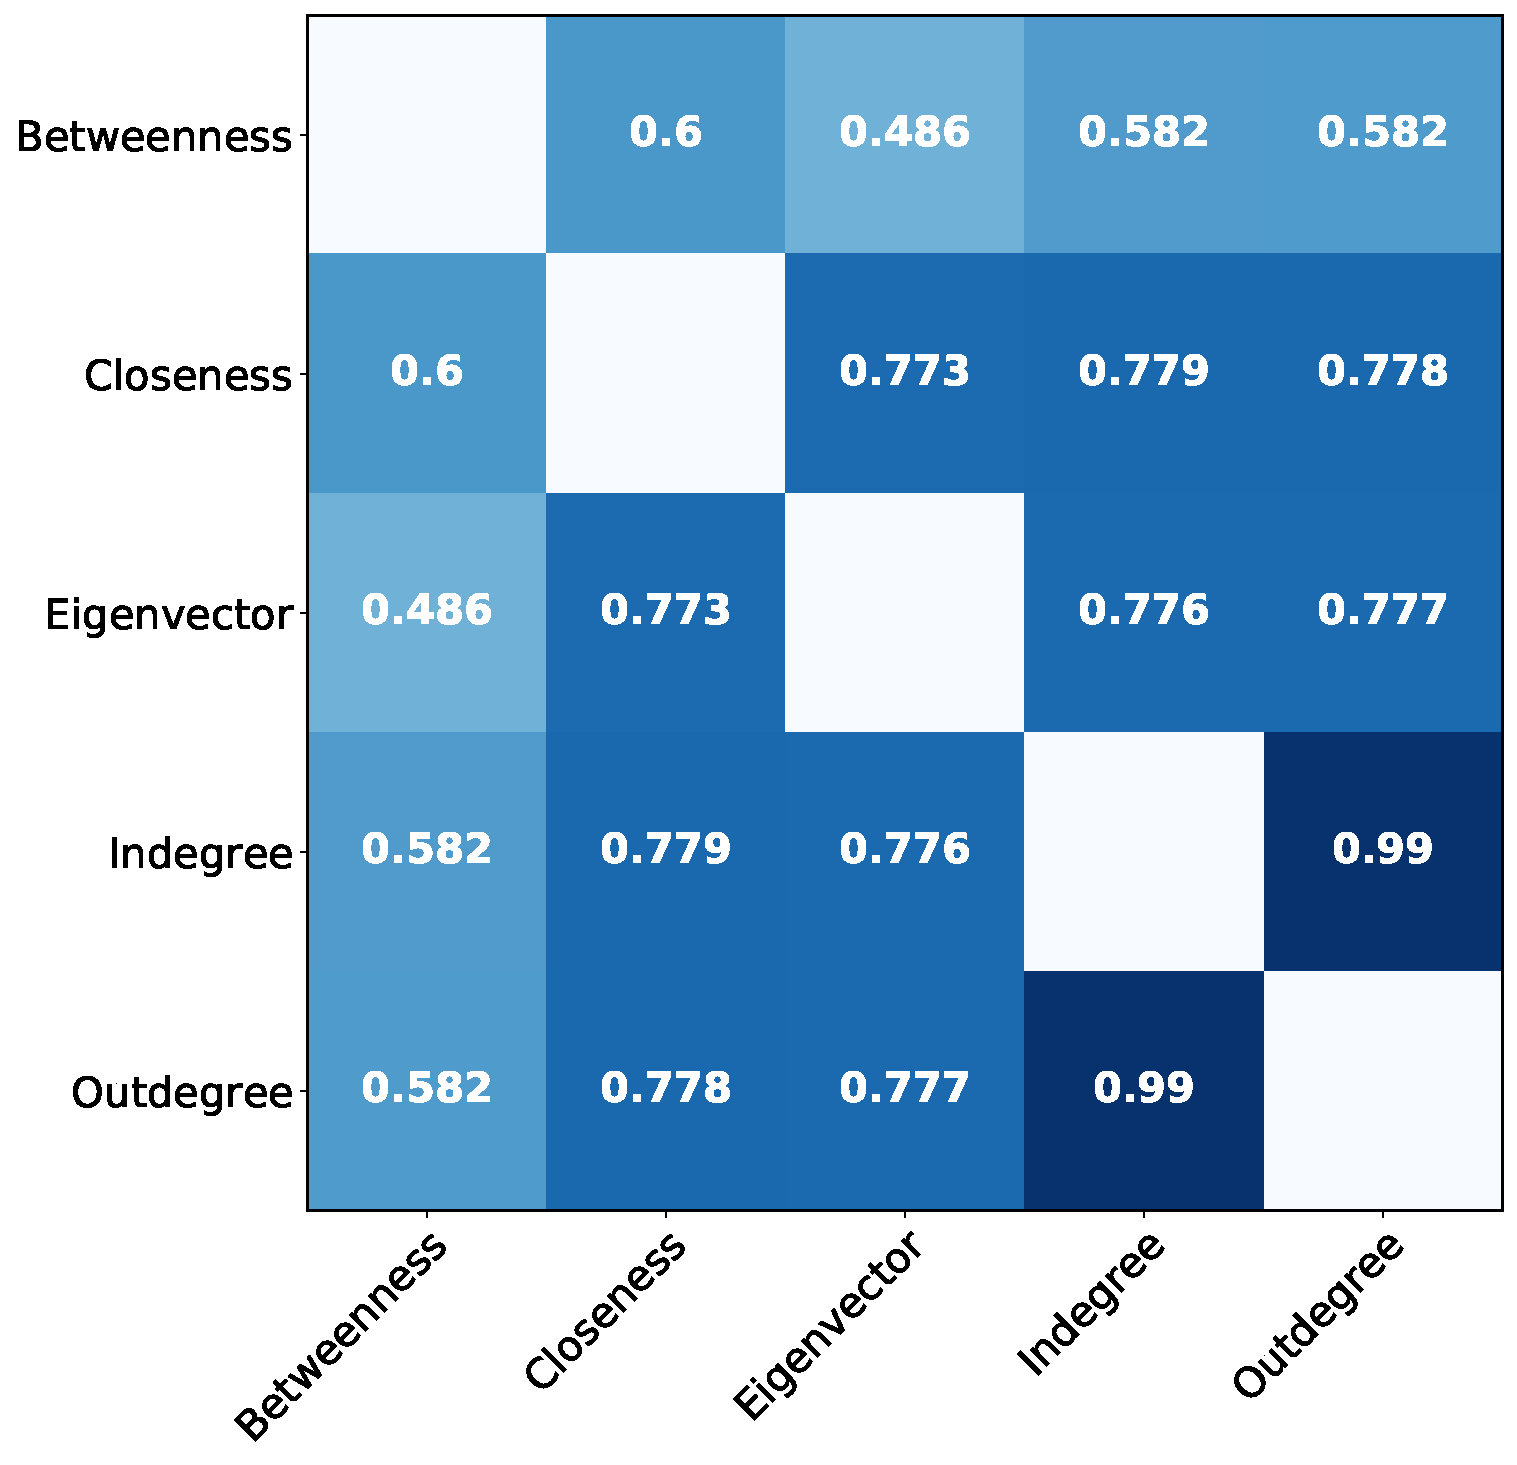
\includegraphics[width=1\textwidth]{Figures/node_remove_overlap_matrix.pdf}
        \caption{Share of nodes}
        \label{fig:node_remove_overlap_matrix}
    \end{subfigure}
    \label{fig:measure_comparison}
\end{figure}
\end{frame}


\begin{frame}{Outcomes of Interest}
\begin{figure}
\begin{center}
    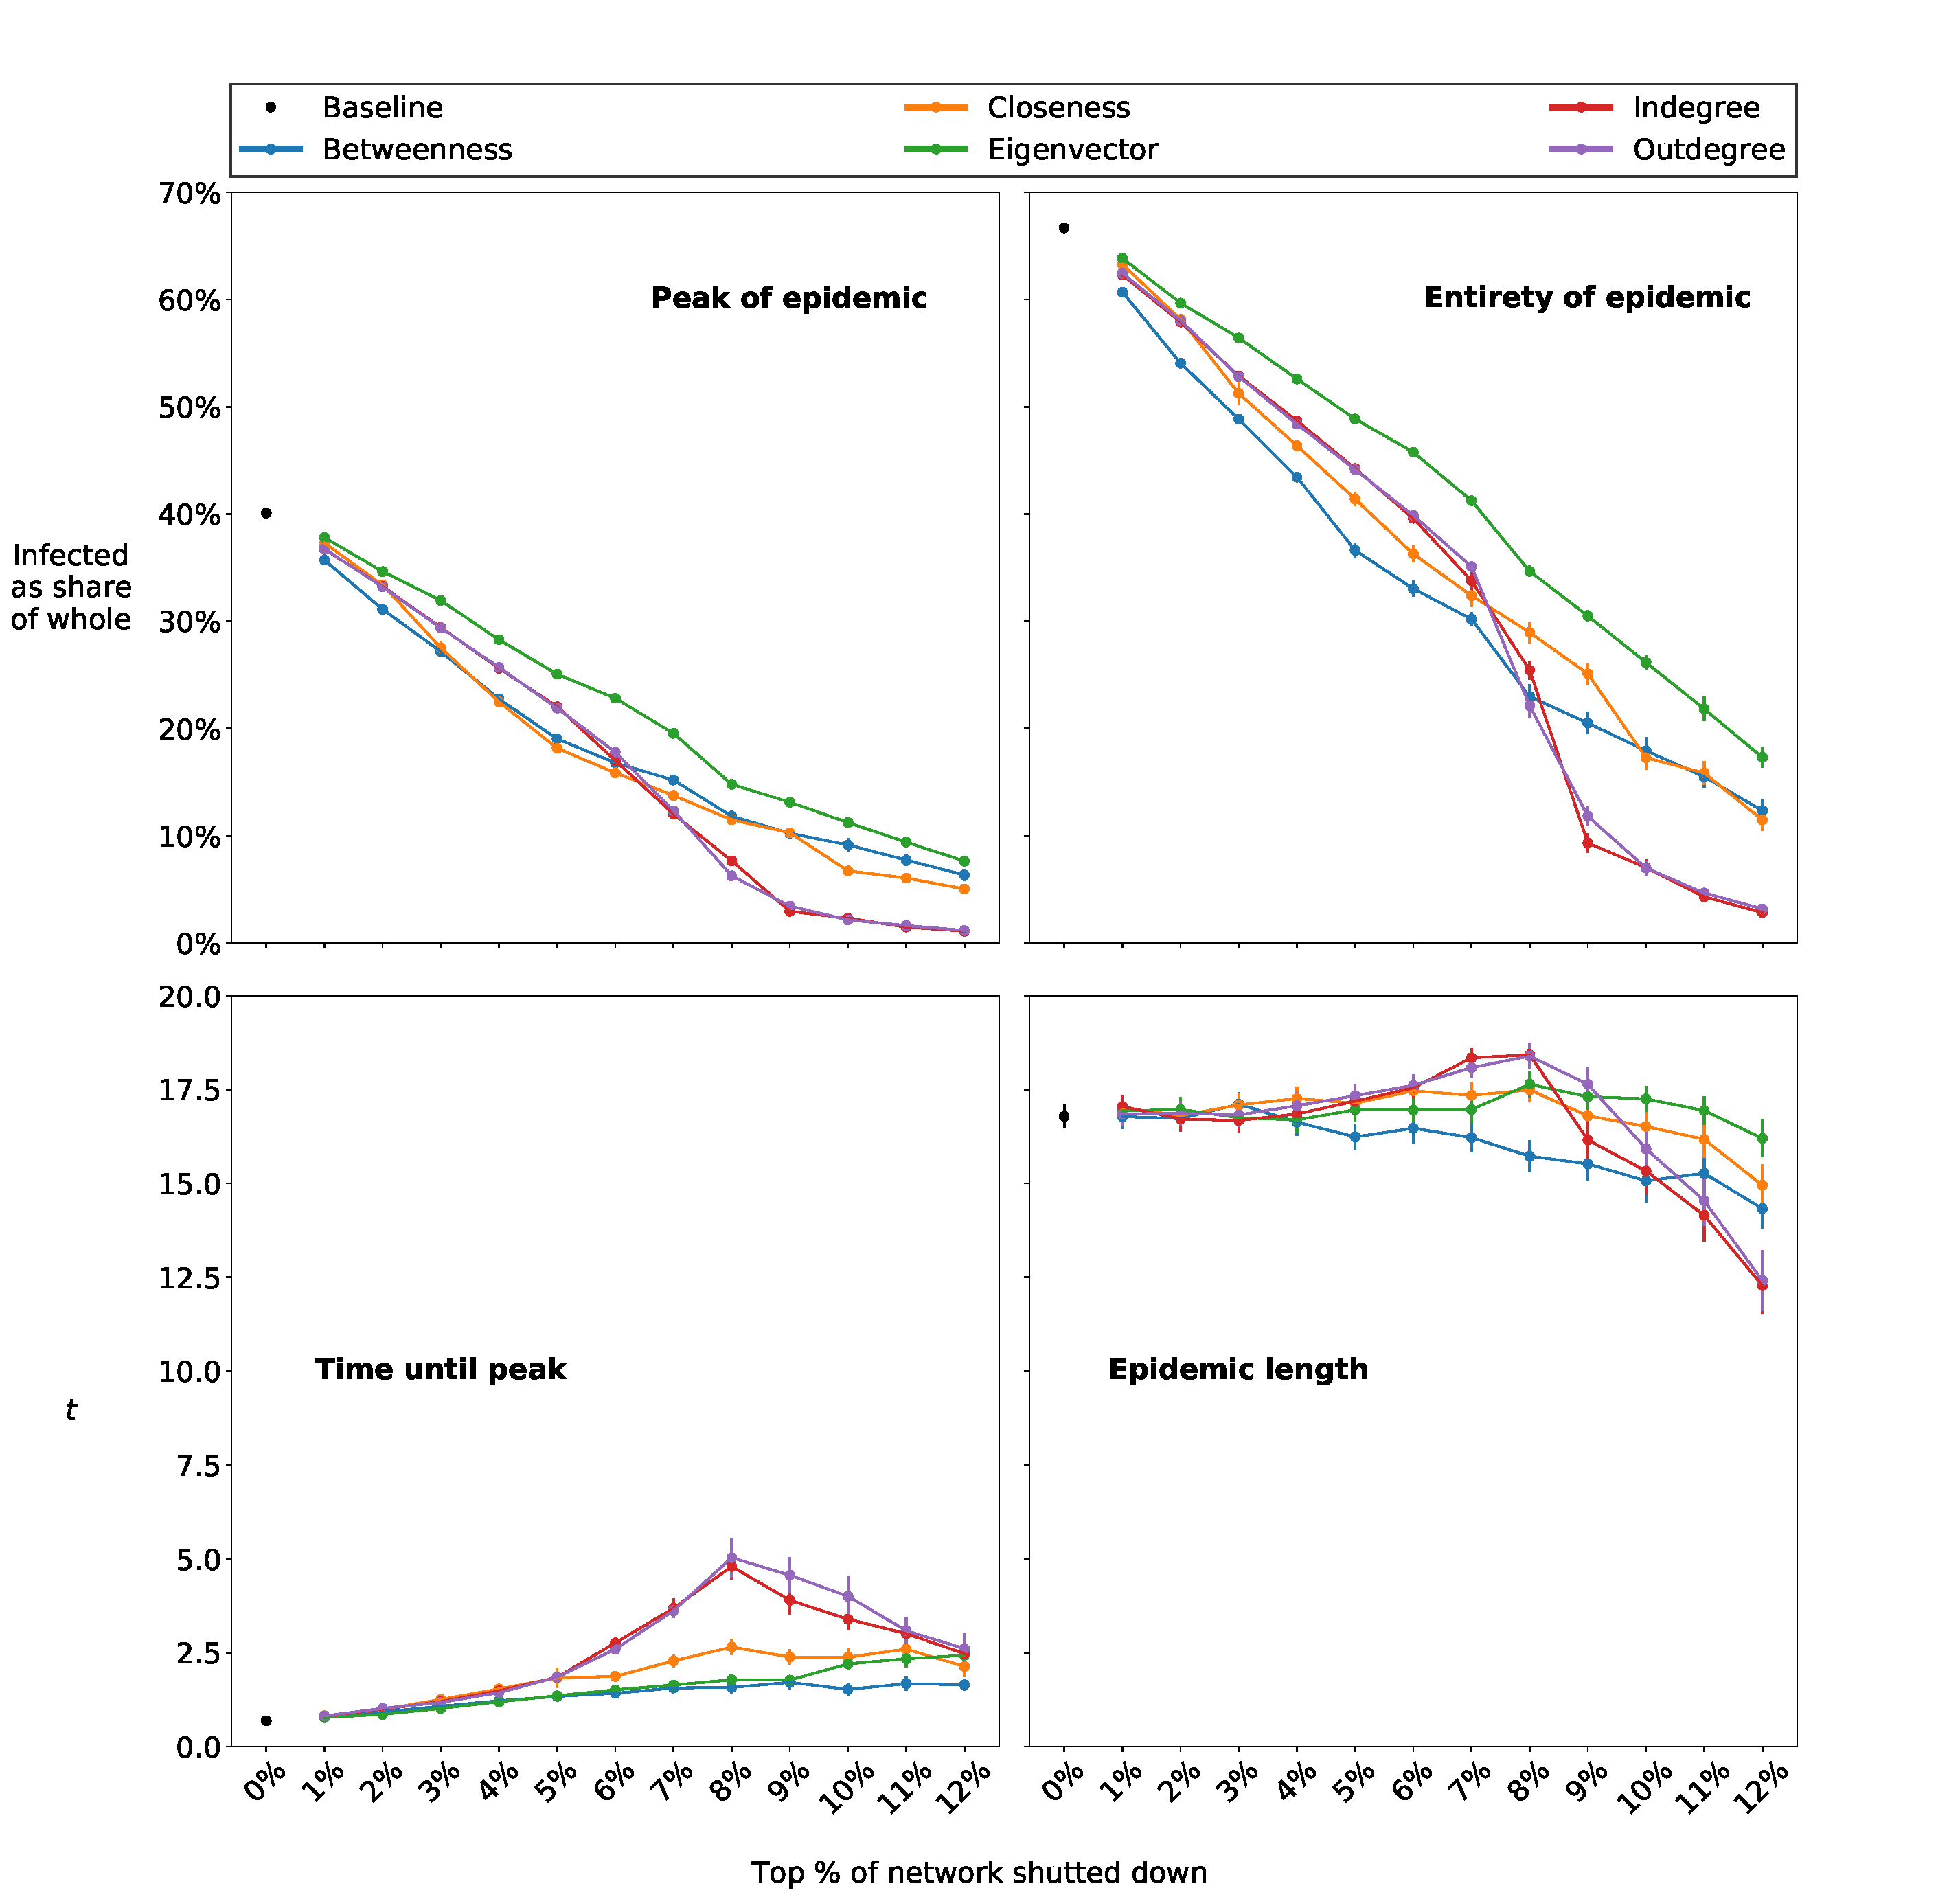
\includegraphics[width=0.75\textwidth]{Figures/interest_outcomes.pdf}
\end{center}
\end{figure}
\end{frame}

%\begin{frame}{Discussion}

 %\begin{itemize}
%     \item assumption: closeness centrality measure most effective - not in general true
 %    \begin{itemize}
 %       \item most effective to reduce the peak 
 %       \item economic state 
 %       \item economic state 
 %   \end{itemize}
     
  %   \begin{itemize}
  %      \item dimensions of pandemic-indicators
  %      \item economical and health factors
 %    \end{itemize}
     
 %   \item Which centrality measures should be taken into account to most effectively contain a pandemic?
%    \begin{itemize}
%        \item BC - minimum closure of airports due to economic pressure 
%        \item DC - more airports need to to be shut down, health care system overburdened 
 %   \end{itemize}
%    \item partly different airports will be shuted down %considering the two different methods
% \end{itemize}
%\end{frame}

\section{Conclusion}
\begin{frame}{Conclusion}
Which centrality measures should be taken into account to most effectively contain a pandemic?
 \begin{itemize}
    \item Depended on dimensions of pandemic-indicators, economical and health factors
    \begin{itemize}
        \item Betweeness centrality - minimum closure of airports due to economic pressure 
        \item Degree centrality - more airports need to to be shut down, health care system overburdened 
    \end{itemize}
    \item Partly different airports will be closed considering the two different methods
 \end{itemize}
\end{frame}
\end{document}
